% Aero Astro template
% Max Opgenoord
% August 2017

\documentclass[unknownkeysallowed,aspectratio=43,10pt,onlymath]{beamer}

% Change the aspect ratio above, the template should adapt (unless you pick some crazy AR)

\usepackage{etex}


\mode<presentation>
{
  \usetheme[nofooter]{AeroAstro}
  \setbeamercovered{transparent}
}

\beamertemplatenavigationsymbolsempty

% Aero Astro template
% Max Opgenoord
% August 2017

% ============================== Tikz ================================== %
% ------------------------------ Packages ------------------------------ %
\usepackage{pgf,pgfpages,pgfplots}
\usepackage{tikz-3dplot}
\usepackage{tkz-euclide}
\usepackage{adjustbox} % Allow for scaling of blocks (especially useful
                       % for tikzpictures)
% ---------------------------------------------------------------------- %

% ------------------------------ Formatting ---------------------------- %
\usetikzlibrary{arrows,shapes,positioning,shadows,trees,patterns,intersections,matrix,fit,backgrounds,automata,calc}
\pgfplotsset{compat=newest}
  \pgfplotsset{plot coordinates/math parser=false}
\newlength\figureheight
    \newlength\figurewidth
\usetkzobj{all}
\tikzset{
basic box/.style = {
    shape = rectangle,
    align = center,
    draw  = #1,
    fill  = #1!25,
    rounded corners},
}
\tikzset{
  invisible/.style={opacity=0},
  visible on/.style={alt={#1{}{invisible}}},
  alt/.code args={<#1>#2#3}{%
    \alt<#1>{\pgfkeysalso{#2}}{\pgfkeysalso{#3}}
  },
}
\tikzset{onslide/.code args={<#1>#2}{%
  \only<#1>{\pgfkeysalso{#2}} % \pgfkeysalso doesn't change the path
}}
% ---------------------------------------------------------------------- %

% ------------------------------ 3D Plots ------------------------------ %
\makeatletter
\tikzoption{canvas is xy plane at z}[]{%
  \def\tikz@plane@origin{\pgfpointxyz{0}{0}{#1}}%
  \def\tikz@plane@x{\pgfpointxyz{1}{0}{#1}}%
  \def\tikz@plane@y{\pgfpointxyz{0}{1}{#1}}%
  \tikz@canvas@is@plane
}
\makeatother
% ---------------------------------------------------------------------- %
% ====================================================================== %

% ============================== Add extra commands ==================== %
% ------------------------------ Misc ---------------------------------- %
\newcommand{\bomega}{\textrm{\boldmath$\omega$}}
\DeclareMathOperator*{\argmin}{arg\,min}
% ---------------------------------------------------------------------- %

% ------------------------------ Partials ------------------------------ %
\newcommand{\PDer}[2]{%
    \frac{\partial #1}{\partial #2}
}
\newcommand{\PDerT}[2]{%
    \frac{\partial^2 #1}{\partial #2^2}
}
\newcommand{\PDerF}[2]{%
    \frac{\partial^4 #1}{\partial #2^4}
}
\newcommand{\PDerFM}[3]{%
    \frac{\partial^4 #1}{\partial #2^2 \partial #3^2}
}
\newcommand{\PDerTh}[2]{%
    \frac{\partial^3 #1}{\partial #2^3}
}
\newcommand{\PDerThM}[3]{%
    \frac{\partial^3 #1}{\partial #2 \partial #3}
}

\newcommand{\PDerM}[3]{%
    \frac{\partial^2 #1}{\partial #2 \partial #3}
}
\newcommand{\DerF}[2]{%
    \frac{\mathrm{d}^4 #1}{\mathrm{d} #2^4}
}
\newcommand{\Der}[2]{%
    \frac{\mathrm{d} #1}{\mathrm{d} #2}
}
\newcommand{\DerT}[2]{%
    \frac{\mathrm{d}^2 #1}{\mathrm{d} #2^2}
}
\newcommand{\DerTh}[2]{%
    \frac{\mathrm{d}^3 #1}{\mathrm{d} #2^3}
}
% ---------------------------------------------------------------------- %
% ====================================================================== %


\addbibresource{bibliography.bib}

\title{Optimal Aircraft Design Decisions Under Uncertainty via Robust Signomial Programming}
\author{Presented by Berk Ozturk, joint work with Ali Saab}
\institute{MIT \\ May 3, 2019}

\begin{document}

{\setbeamertemplate{footline}{}%
\begin{frame}[t]\titlepage\end{frame}%
\addtocounter{framenumber}{-1}}

\section*{Background} % "*" prevents a full-page section slide to show

\begin{frame}{Motivation}

Most Latex beamer templates have a lot of noise on the slides and are not focused on content.\\ \ \\

You can use this template to generate slides focused on content to help get the message across.
Remember, however, a template is only a small part of making a good presentation.

\end{frame}

\section{Template}

\begin{frame}{Citations}
Cite something using.\mcite{theodorsen1935general}
The full reference will show up at the end of the presentation.
If a DOI, URL, or ISBN is available, the title of the footnote will be a hyperlink to the paper. Like so\mcite{opgenoord2017physics}.

\end{frame}

\subsection{Subsections}

\begin{frame}{A word about subsection title pages}

In older versions of \LaTeX{}, you need to have used at least one \texttt{\textbackslash section} command, before you can use the \texttt{\textbackslash section} command.
However, as of the 2017 version, this seems fixed.

\end{frame}

\subsection*{Same thing} % Star does same thing as for section pages

\begin{frame}{Suppressing subsection title pages}

Using the command \texttt{\textbackslash subsection*} will prevent the subsection title page from showing (this works in exactly the same way as for sections).

\end{frame}

\begin{frame}{Note on itemize}

You can use \texttt{\textbackslash begin\{itemize\} \textbackslash item ... \textbackslash end\{itemize\}} to itemize list, which will look like
\begin{itemize}
\item Itemize is great
\item Or is it?
\end{itemize}

In general, however, you do not necessarily need to have the bullets -- in fact, they can be distracting. In that case, you want to use \texttt{\textbackslash begin\{itemize\} \textbackslash item[] ... \textbackslash end\{itemize\}}, which will look like
\begin{itemize}
\item[] Much cleaner
\item[] And you still have proper spacing
\end{itemize}

Finally you can also use \texttt{\textbackslash begin\{items\} \textbackslash item[] ... \textbackslash end\{items\}} if you want slightly more spacing between different items
\begin{items}
\item So much
\item space
\end{items}

\end{frame}

\begin{frame}{Enumerate}

Again, in general there is no need to add numbers, but you can use \texttt{\textbackslash begin\{enumerate\} \textbackslash item ... \textbackslash end\{enumerate\}}, if you really want to.
\begin{enumerate}
\item Important thing
\item Other important thing
\end{enumerate}

Again, you can also use \texttt{\textbackslash begin\{enums\} \textbackslash item ... \textbackslash end\{enums\}} if you want slightly more spacing between different items
\begin{enums}
\item So much
\item space
\end{enums}

\end{frame}

\begin{frame}{Some math}

  Be careful with adding too much math on a slide!

  \begin{subequations}
    \begin{align*}
      \Delta L_{nc}(t) &= \frac{1}{4} \rho_{\infty} \pi c^2 \left[ \Delta \ddot{h} - \left(x_{ea} - \frac{c}{2}\right) \Delta \ddot{\theta} \right] + \frac{1}{4}\rho_{\infty} \pi c^2 V_{\!\infty} \Delta\dot{\theta}  \\
      \Delta M_{nc}(t) &= \frac{1}{4} \rho_{\infty} \pi c^2 \left( x_{ea} - \frac{c}{2}\right) \left[\Delta\ddot{h}
      - \left(x_{ea} - \frac{c}{2}\right) \Delta \ddot{\theta}\right] - \frac{\rho_{\infty} \pi c^4}{128} \Delta\ddot{\theta} \\
      & \quad - \frac{1}{4} \rho_{\infty} \pi c^2 V_{\infty} \left(\frac{3}{4} c - x_{ea}\right) \Delta \dot{\theta}
    \end{align*}
  \end{subequations}

\end{frame}

\begin{frame}{Handouts}

  In general, sending out slides is not a great idea, because quite a lot of the nuance is lost by only seeing slides. \\ \ \\

  However, if you have to send out slides, it is usually a better idea to send a handout, where the first slide is the abstract of the talk and information about the talk is added to each slide.
  You can also add copyright information to this handout. \\ \ \\

  An example is found in the \texttt{handout} folder.

\end{frame}

\secimage{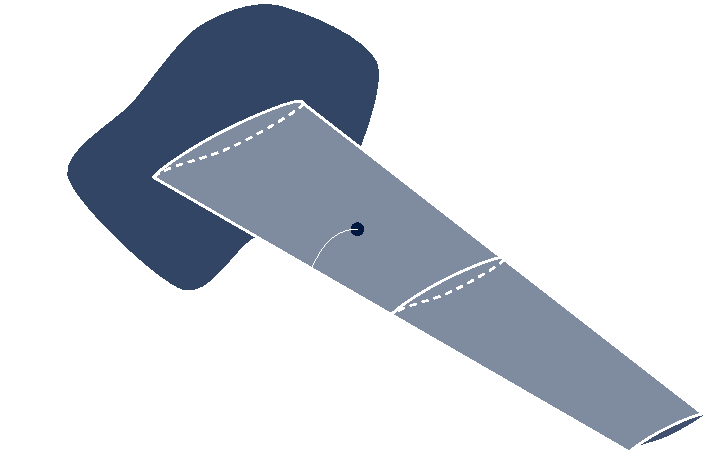
\includegraphics[width=0.75\linewidth]{figures/windtunnel}}

\section{Results}

\begin{frame}{Noticed the picture on section slide?}
  I use this to help with transition. It can be used to quickly show a setup that you use for results, for instance.
  You can redefine it before each section using \texttt{\textbackslash secimage} or \texttt{\textbackslash subsecimage}. By default it is empty.
\end{frame}

\begin{frame}{Best results}

Don't \alert{ever} use figure captions in presentations, instead use minipages. In general, minipages are a good idea to position text and figures on slides. For really intricate slides layouts, use \texttt{tikzpictures}.

\begin{minipage}{0.485\textwidth}

\includegraphics[width=\linewidth]{figures/logos/AeroAstroDB}
\end{minipage}\hfill
\begin{minipage}{0.485\textwidth}

\includegraphics[width=\linewidth]{figures/logos/AeroAstroDB}
\end{minipage}

\end{frame}

\begin{frame}{Drawing figures in Tikz}

  Below is an example of a figure drawn with Tikz.
  The source code can be found in \texttt{figures\textbackslash clcd}.
  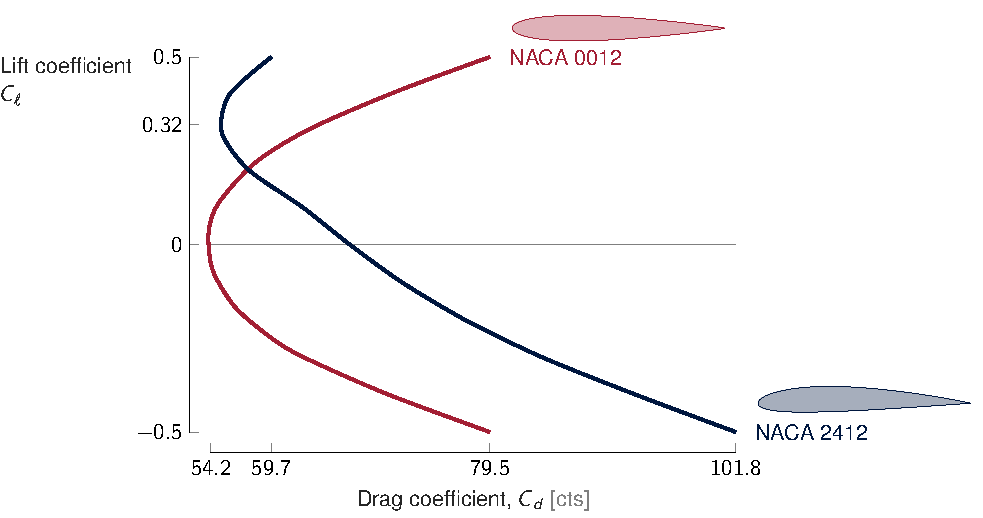
\includegraphics[width=\linewidth]{figures/clcd/clcd}

  Note that this is a not an all-encompassing solution to figures.
  Each figure needs to be tailored to the specific message that you are trying to get across.


\end{frame}

\begin{frame}{Scaling of tikzpictures}

\texttt{tikz} is great for making vector graphics, but you may want to scale the graphic without changing all the coordinates in your drawing. There are two ways you can handle that.
\begin{enumerate}
  \item Generate the \texttt{tikzpicture} in a \texttt{standalone} \TeX{} document and include it using \texttt{\textbackslash includegraphics} and scale appropriately. This also reduces compile time.
  \item Use \texttt{adjustbox} to scale your figure inside a document, an example of which is shown below.
\end{enumerate}

\begin{minipage}{0.485\textwidth}
  \centering
  \begin{tikzpicture}
    \draw[black,thick,fill=AAblue!50] (0,0) -- (2,0) -- (0,2) -- cycle;
  \end{tikzpicture}
\end{minipage}\hfill
\begin{minipage}{0.485\textwidth}
  \centering
  \begin{adjustbox}{max width = 0.1\textwidth,max height = 0.1\textheight}
  \begin{tikzpicture}
    \draw[black,thick,fill=AAblue!50] (0,0) -- (2,0) -- (0,2) -- cycle;
  \end{tikzpicture}
  \end{adjustbox}
\end{minipage}

\end{frame}

\secimage{ }
\section{Message}

\begin{frame}{Use the heading of a slide\\ to write down the message}

And remember: everything you put on the slides needs to support the main message. Anything else is noise.


\end{frame}

\begin{framedark}[t]{Important Presentation}
\vspace{-0.025\textheight}
\textcolor{AAlb}{\underline{Max Opgenoord}, John Doe}

\vspace{0.2\textheight}

\textcolor{AAlb}{\textbf{Summary}}
\medskip
\begin{itemize}
\item[] I usually finish my presentation on a summary slide (in dark) instead of just a ``Thank You" slide
\end{itemize}
\bigskip
\textcolor{AAlb}{\textbf{Future}}
\medskip
\begin{itemize}
\item[] Presentations focused on content
\end{itemize}
\end{framedark}

%% Bibliography
\appendix
\setbeamertemplate{footline}[emptyapp]
\section*{References}
\begin{frame}[t,allowframebreaks]
\frametitle{References}
{\scriptsize
 \printbibliography%
}
\end{frame}

\begin{frame}{Back-up material}

\end{frame}


\end{document}
